\documentclass[12pt]{article}

\usepackage{graphicx}
\usepackage{amsmath,amssymb}
\usepackage{mathptmx}
\usepackage{hyperref}
\usepackage{xcolor}
\usepackage[margin=1in]{geometry}
\usepackage{setspace}
\onehalfspacing

\hypersetup{
  colorlinks=true,
  linkcolor=blue!60!black,
  citecolor=blue!60!black,
  urlcolor=blue!60!black
}

\begin{document}

\title{A Pedagogical Introduction to the Architecture of Claude\\for Research Administrators}

\author{Duncan A. Brown\\[6pt]
\textit{Office of Research, Lyman Hall, Syracuse University, Syracuse NY 13244}\\[4pt]
Corresponding author: Duncan A. Brown, \href{mailto:dabrown@syr.edu}{dabrown@syr.edu}}

\date{}

\maketitle
\begin{abstract}
Large language models (LLMs) such as Claude are increasingly used in research administration for data analysis, document generation, and institutional research. However, their internal architecture is poorly understood by most users, leading to misplaced trust in some outputs and unnecessary skepticism toward others. While a growing literature addresses AI literacy for students and the general public, little work has focused on the specific architectural knowledge that domain professionals need in order to use LLM-based systems effectively and safely. This paper provides a scaffolded introduction to the architecture of Claude, Anthropic's large language model, aimed at research administrators and other professionals who use these tools but lack a machine learning background. We begin with a concrete analogy between Claude's runtime and a traditional Python program, then progressively introduce the context window, chat persistence, projects, skills, connectors, the sandboxed execution environment, the orchestration harness, the research tool, and finally the tokenizer and transformer architecture. Each section builds on concepts from previous sections, and the paper is designed so that readers can stop at the level of detail that serves their needs. We emphasize the practical implications of the architecture for the trustworthiness of different types of output, particularly the distinction between statistical text generation and deterministic code execution. To our knowledge, this is the first detailed architectural description of a production LLM system written for a non-technical professional audience, derived in part from direct runtime inspection. Appendix~\ref{app:osp} provides a detailed case study of a production skill used for sponsored research budget development at Syracuse University.
\end{abstract}

\noindent\textbf{Keywords:} AI literacy, large language models, human-AI interaction, research administration, system architecture

\section{Introduction}
\label{sec:intro}

Claude is a large language model (LLM) developed by Anthropic. When accessed through the Claude web interface, mobile application, or desktop application, Claude can converse in natural language, write and execute code, search the web, read and create documents, and interact with external services through authenticated connectors. It is increasingly used in research administration for tasks ranging from budget analysis to policy drafting to institutional data visualization.

Despite this widespread use, most users---including sophisticated professionals in research administration and finance---have little understanding of how Claude actually works. This lack of understanding creates two practical problems. First, users may trust outputs that should not be trusted, particularly numerical results that the model generates statistically rather than computing deterministically. Second, users may fail to take advantage of the system's actual capabilities because they do not understand what it can and cannot do.

A growing body of human-computer interaction (HCI) research has identified AI literacy as a critical competency for effective human-AI interaction~\cite{long2020ai,ng2021ai}, and recent work has documented the specific ways that non-expert users struggle with LLM-based systems~\cite{zamfirescu2023johnny,tankelevitch2024metacognitive}. However, the AI literacy literature has focused primarily on K--12 and undergraduate education, and the resources available to working professionals tend toward either surface-level overviews (``it's a neural network'') or inaccessibly technical accounts (research papers assuming graduate-level machine learning background). This paper addresses the gap between these extremes by providing a detailed, scaffolded architectural description of a production LLM system, written for domain professionals who need to make trust decisions about specific types of output. Section~\ref{sec:related} discusses related work in more detail.

This paper provides a pedagogical introduction to Claude's architecture, motivated by conversations between the author and the Senior Vice President and Chief Financial Officer at Syracuse University.

Before proceeding to the technical details, we highlight several practical takeaways that are developed fully in Sec.~\ref{sec:implications} but that even casual users should keep in mind. Most importantly, \emph{never trust a number that Claude produced in prose}: the model predicts plausible-looking tokens rather than computing results, so all financial analysis should be routed through deterministic code execution. Second, Claude cannot reliably report on its own architecture or internal state; when one model instance was asked how many tokens remained in its context window, it fabricated a precise answer complete with a fictional claim about receiving ``token usage warnings.'' Third, every message, tool call, and loaded skill consumes tokens from a finite context window, so long conversations eventually degrade. Fourth, conversations are bound to a specific model version and cannot be transferred between models. Finally, Claude's Research tool (Sec.~\ref{sec:research}) can conduct extended multi-source investigations that run for up to 45 minutes---a capability that many users are unaware of.

The explanations here are scaffolded: each section introduces new concepts by building on the previous section's vocabulary. Section~\ref{sec:related} reviews related work on AI literacy and user understanding of LLMs. Section~\ref{sec:analogy} introduces Claude by analogy to a traditional Python program. Section~\ref{sec:context} explains the context window. Section~\ref{sec:chats} explains chat persistence and model binding. Sections~\ref{sec:projects} and~\ref{sec:skills} describe projects and skills. Section~\ref{sec:mcp} introduces connectors and the Model Context Protocol. Section~\ref{sec:container} describes the sandboxed execution environment. Section~\ref{sec:harness} explains the orchestration harness. Section~\ref{sec:compaction} describes compaction. Section~\ref{sec:research} describes the research tool. Sections~\ref{sec:tokenizer} and~\ref{sec:transformer} introduce the tokenizer and transformer. Section~\ref{sec:implications} discusses practical implications. Readers should feel free to stop at whatever level of detail serves their needs; the first nine sections provide a complete working understanding for most practical purposes. Appendix~\ref{app:osp} provides a detailed case study of a production skill.

\section{Related work}
\label{sec:related}

Long and Magerko~\cite{long2020ai} define AI literacy as ``a set of competencies that enables individuals to critically evaluate AI technologies; communicate and collaborate effectively with AI; and use AI as a tool online, at home, and in the workplace.'' Their framework identifies 17 competencies, including the ability to distinguish what AI can and cannot do, understand how data and algorithms shape outputs, and recognize the difference between AI intelligence and human intelligence. Ng et al.~\cite{ng2021ai} synthesize this and related work into four aspects of AI literacy: knowing and understanding AI, using and applying AI, evaluating and creating with AI, and attending to ethical issues.

Most AI literacy research has focused on K--12 and undergraduate settings. Far less attention has been paid to the needs of working professionals who use LLM-based tools as part of their daily work but who lack the time or background for a formal machine learning course. This gap is consequential: Zamfirescu-Pereira et al.~\cite{zamfirescu2023johnny} found that non-expert users struggle with LLM prompting in ways that parallel known difficulties in end-user programming, including opportunistic rather than systematic exploration and poor mental models of system capabilities. Tankelevitch et al.~\cite{tankelevitch2024metacognitive} argue that generative AI systems impose substantial \emph{metacognitive} demands on users---requiring self-awareness of task goals, calibrated confidence in output evaluation, and strategic decisions about when and how to delegate to AI---and that these demands are poorly supported by current system designs.

The present paper is situated at the intersection of these concerns. Rather than proposing a general AI literacy framework, we provide the specific architectural knowledge that a domain professional needs in order to make informed trust decisions about LLM outputs: which outputs are generated statistically, which are computed deterministically, where persistent state exists and where it does not, and how the various components of a production LLM system interact. This is closer in spirit to a technical reference than to a curriculum, but it is written at a level of detail that assumes no prior knowledge of machine learning. We are not aware of comparable work providing this level of architectural detail about a production LLM system for a non-technical professional audience.

\section{Claude by analogy to traditional software}
\label{sec:analogy}

Consider a traditional software stack, illustrated on the left side of Fig.~\ref{fig:stack}. At the bottom is a filesystem that stores data and programs. Above it is an operating system (OS) that manages hardware resources and executes system calls. Above the OS is a language interpreter---say, a Python interpreter---that executes code written by the user. At the top is the user, who writes Python commands and receives deterministic results: \texttt{2 + 2} always returns \texttt{4}.

\begin{figure}
\centering
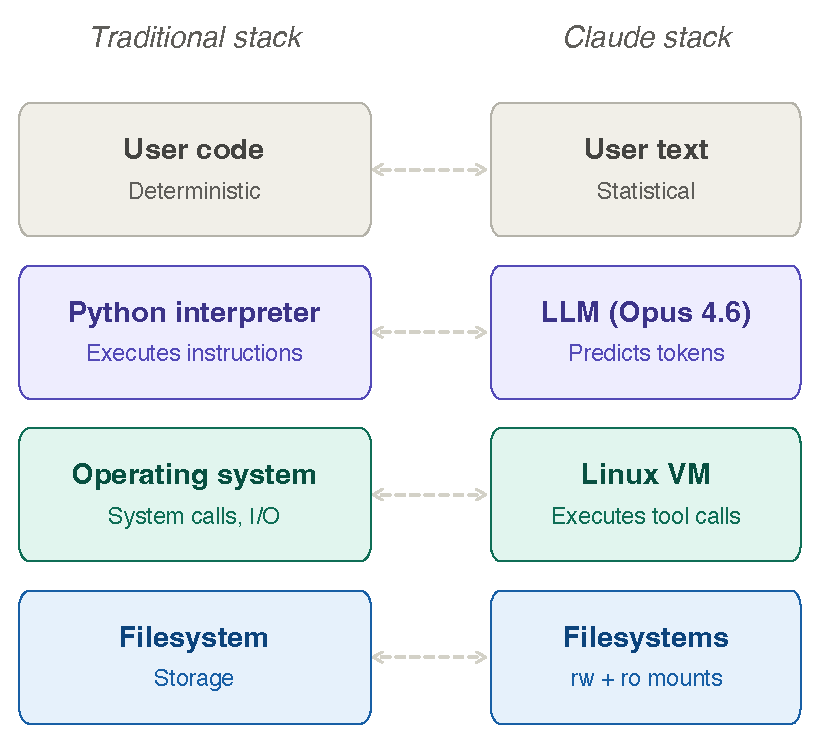
\includegraphics[width=0.48\textwidth]{fig_stack.pdf}
\caption{Layer analogy between a traditional software stack (left) and the Claude stack (right). Each layer has a functional analogue. The critical difference is at the interpreter layer: Python executes deterministic instructions; the LLM generates statistically probable token continuations.}
\label{fig:stack}
\end{figure}

Claude has an analogous layered architecture, shown on the right side of Fig.~\ref{fig:stack}. At the bottom are filesystems (some read-write, some read-only). Above them is a Linux virtual machine (VM) that can execute shell commands, Python scripts, and other code. Above the Linux VM is the LLM itself---an Opus 4.6 or Sonnet 4.6 model---which is analogous to the Python interpreter. At the top is the user, who writes natural language text rather than Python code. The critical difference is at the interpreter layer. When you type \texttt{print(2 + 2)} into a Python interpreter, the result is \emph{always} \texttt{4}. The interpreter executes a deterministic algorithm. When you type ``What is 2 + 2?'' into Claude, the LLM generates a response by predicting the most statistically probable continuation of the input text, based on patterns learned during training. For simple arithmetic, the prediction is almost certainly ``4,'' because that answer appears overwhelmingly in the training data. But the mechanism is fundamentally different: the LLM is not performing addition. It is predicting tokens. For more complex calculations, this distinction has real consequences, as discussed in Sec.~\ref{sec:implications}.

The analogy extends further. A Python interpreter can import libraries to extend its capabilities; the LLM can load \emph{skills} (Sec.~\ref{sec:skills}). A Python program can call external processes; the LLM can issue \emph{tool calls} that execute code on the Linux VM (Sec.~\ref{sec:container}). A Python process maintains state in memory between commands; the LLM does not---but it creates the \emph{illusion} of continuity through a mechanism called the context window (Sec.~\ref{sec:context}).

\section{The context window}
\label{sec:context}

The most important architectural concept for understanding Claude is the \emph{context window}. The context window is the complete text that the model processes on each turn of conversation. It includes the system prompt (Anthropic's instructions to the model), the user's preferences, project instructions, conversation history (every message exchanged between the user and Claude in the current chat), and the results of any tool calls. For Claude Opus 4.6 and Sonnet 4.6, the context window can hold approximately one million tokens~\cite{anthropic_api_docs}, where a token is roughly three-quarters of an English word.

The context window is not persistent memory. It is reconstructed from scratch on every turn. When the user presses ``return'' after typing a message, the orchestration system (Sec.~\ref{sec:harness}) assembles the complete context---system prompt, preferences, project instructions, conversation history including the new message---and feeds the entire sequence through the model. The model generates its response, and that response is appended to the conversation history. On the \emph{next} turn, the entire conversation history, now including both the user's latest message and the model's response, is fed through the model again from the beginning.

This is the respect in which the Python analogy breaks down most instructively. Consider a file called \texttt{context.py}. When the user types a message, it is appended to \texttt{context.py}. The interpreter runs the entire file and appends its output to the file. On the next turn, the interpreter runs the \emph{entire} file again---including all previous inputs and outputs---and appends new output. The file grows monotonically. There is no separate memory of previous runs; everything the interpreter knows must be in the file. This has several important consequences:

\begin{enumerate}
\item \textbf{No persistent state.} Claude does not remember previous turns the way a person remembers earlier parts of a conversation. It has access to the \emph{text} of previous turns because that text is included in the context window, but it processes the entire conversation afresh each time.

\item \textbf{Finite capacity.} The context window has a hard limit (approximately one million tokens for the current models). As the conversation grows, the total context approaches this limit. Section~\ref{sec:compaction} describes what happens when this limit is reached.

\item \textbf{Monotonic growth.} Every tool call result, every message, and every response adds tokens to the context window that persist for the rest of the conversation. This is illustrated schematically in Fig.~\ref{fig:context_growth}.
\end{enumerate}

\begin{figure}
\centering
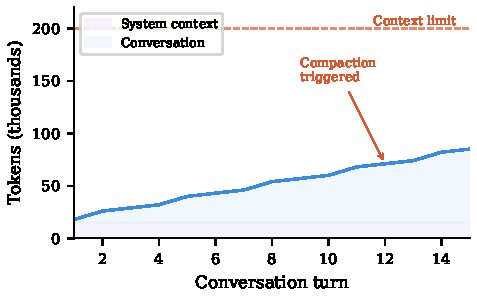
\includegraphics[width=0.48\textwidth]{fig_context_growth.pdf}
\caption{Schematic illustration of context window growth. The lower (purple) region represents fixed overhead (system prompt, preferences, project instructions). The upper (blue) region represents cumulative conversation history. Tool-using turns add more tokens than text exchanges. When the total approaches the limit, compaction (Sec.~\ref{sec:compaction}) is triggered.}
\label{fig:context_growth}
\end{figure}

\section{Chats, models, and persistence}
\label{sec:chats}

A common misconception is that a Claude conversation ``ends'' when the user closes the browser tab. In fact, chats are persistent. When a user clicks ``New chat,'' the previous chat is saved, and the user can return to it at any time, scroll through the full history, and continue the conversation by typing a new message. At that point, the system reconstructs the context window from the saved history and proceeds exactly as described in Sec.~\ref{sec:context}. From the model's perspective, there is no difference between two messages thirty seconds apart and two messages a week apart.

A chat persists until the user explicitly deletes it, or until Anthropic retires the specific model version the chat was created with. This second condition is important: each chat is \emph{bound to a specific model version}. A conversation started with Sonnet 4.6 can only be continued with Sonnet 4.6. The user cannot resume that conversation using Opus 4.6, even though both models belong to the same family. The reason is architectural. Each model has its own tokenizer (Sec.~\ref{sec:tokenizer}) and different trained weights that produce different probability distributions over output tokens. A conversation history is not just text; it is a sequence of exchanges generated by a \emph{specific} model. Feeding that history into a different model could produce incoherent results. To move content between models, the user must manually extract information (copying text or downloading files) and paste it into a new chat---analogous to exporting data from one program and importing it into another.

``Starting a new chat'' means starting with a fresh context window. No conversation history carries over. The execution container (Sec.~\ref{sec:container}) is a new instance with a clean filesystem. The only information that persists across chats---other than project files and skills---is Anthropic's \emph{memory} system, which extracts key facts from conversations and injects them into future context windows. Memory is a curated summary, not a complete transcript.

\section{Projects}
\label{sec:projects}

A \textbf{project} is a persistent workspace that provides structure and context across multiple chats. Projects serve as the organizational unit for serious analytical work, and understanding their capabilities is essential for effective use of Claude in research administration. A project consists of three components. First, \emph{project instructions}: a natural language document describing the project's purpose, data sources, analysis requirements, and behavioral guidelines. These instructions are injected into the context window on every turn of every chat within the project, ensuring consistent behavior regardless of which specific chat the user is working in. For example, the Syracuse University research data analysis project includes instructions specifying which data files are available, how to parse Tableau exports with merged cells, and which analysis tools to use for different types of queries. Second, \emph{uploaded data files}, stored on a read-only filesystem at \texttt{/mnt/project} and accessible to all chats in the project. Third, \emph{user-defined skills} (Sec.~\ref{sec:skills}), which extend the model's capabilities for domain-specific tasks. Projects provide several capabilities beyond simple file storage:

\begin{enumerate}
\item \textbf{Cross-chat search.} A chat within a project can search the content of other chats in the same project. This means that analytical work done in one chat---a budget analysis, a data query, a policy discussion---can be retrieved and referenced from a different chat without the user needing to copy and paste.

\item \textbf{Project-scoped memory.} Each project maintains its own memory space, separate from the user's global memory and from other projects. Facts extracted from chats within a project are available to future chats in that project but do not leak into unrelated work.

\item \textbf{Information firewalling.} Chats within a project cannot access chats outside the project, and vice versa. This provides a degree of information separation: a project containing sensitive budget data will not have its contents surface in an unrelated conversation about, say, travel planning. This separation is not a security boundary in the cryptographic sense, but it provides practical compartmentalization.

\item \textbf{Consistent analytical environment.} Because project instructions load on every turn, the model's behavior within a project is consistent. A query about research expenditures in a fresh chat within the research data project will follow the same analytical protocols as a query in a months-old chat in the same project.
\end{enumerate}

\section{Skills}
\label{sec:skills}

A \textbf{skill} is a structured package that extends the model's capabilities for a specific task. Where project instructions provide context and guidelines, skills provide \emph{capability}---the ability to perform complex, domain-specific operations that the base model cannot do reliably on its own. Skills are packaged as zip files and stored on a read-only filesystem at \texttt{/mnt/skills}. Internally, a skill contains up to four components, illustrated in Fig.~\ref{fig:skill}:

\begin{figure}
\centering
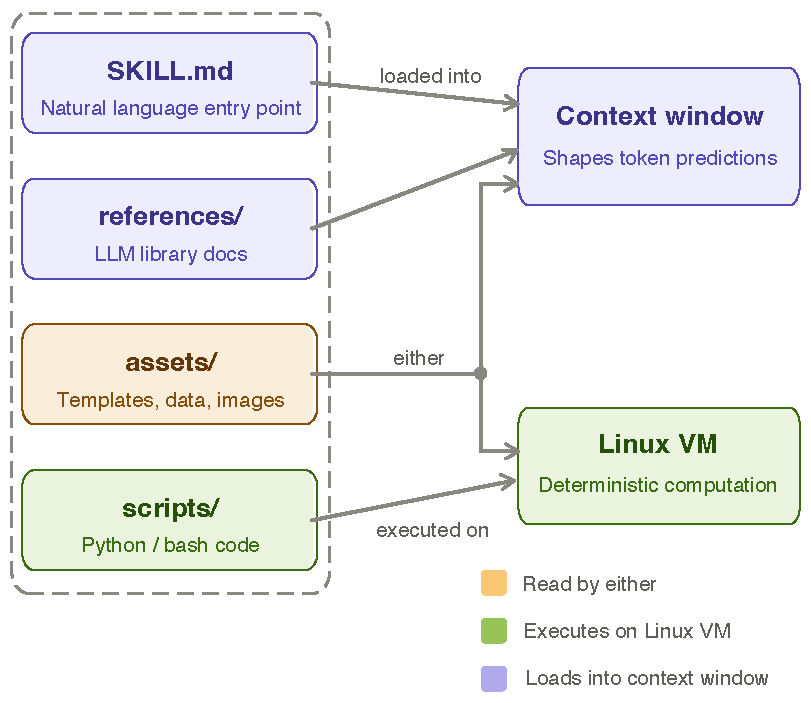
\includegraphics[width=0.48\textwidth]{fig_skill.pdf}
\caption{Anatomy of a Claude skill. A skill is a zip file containing up to four components shown inside the dotted box. SKILL.md serves as the entry point and is loaded into the LLM's context window. The scripts directory contains deterministic code for the Linux VM. The references and assets directories provide additional documentation and data files. Not all skills contain all four components.}
\label{fig:skill}
\end{figure}

\begin{enumerate}
\item \texttt{SKILL.md}: A markdown file containing natural language instructions. This is the entry point of the skill. When loaded into the context window, its instructions shape the model's behavior---not by being executed sequentially, but by changing the probability distribution over the model's output tokens. It is analogous to the \texttt{main()} function of a program, but written in English rather than code.

\item \texttt{references/}: Additional documentation that can be loaded into the context window. These serve as ``library documentation'' that the model consults when needed. For example, a budget skill might include reference files on NIH salary cap policies, NSF cost-sharing rules, and fringe rate tables.

\item \texttt{scripts/}: Python or bash code that executes \emph{deterministically} on the Linux VM when the model issues a tool call. These scripts perform data loading, computation, and file manipulation---tasks where statistical prediction would be unreliable. For example, a budget skill includes scripts for looking up fringe rates, calculating fully loaded salary costs, and populating Excel workbook templates.

\item \texttt{assets/}: Supporting files used by the scripts, such as Excel templates, per diem rate tables, or reference images.
\end{enumerate}

Skills are not loaded automatically. Because the context window has finite capacity (Sec.~\ref{sec:context}), loading a skill consumes tokens that are then unavailable for conversation. The model loads only the skills relevant to the current query, analogous to how a Python program imports only the libraries it needs.

Skills are not written in a text editor the way a programmer writes Python code. Instead, they are created through an interactive process with an LLM instance, using a meta-skill called the \emph{skill-creator}~\cite{anthropic_api_docs}. The process, illustrated in Fig.~\ref{fig:skill_lifecycle}, works as follows:

\begin{figure}[htbp]
\centering
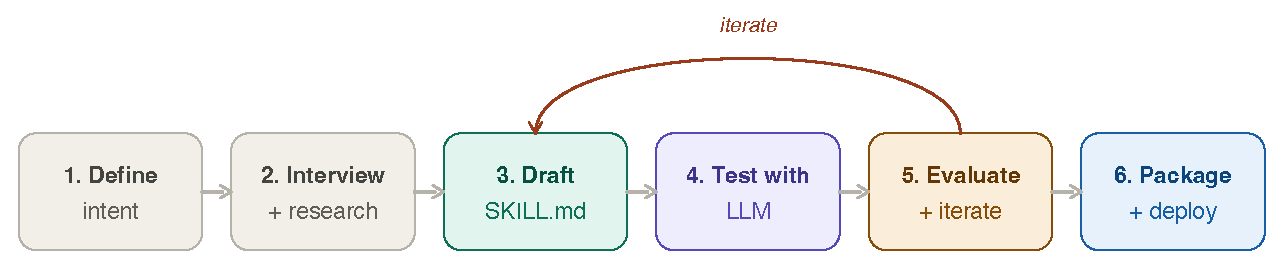
\includegraphics[width=0.95\textwidth]{fig_skill_lifecycle.pdf}
\caption{Skill development lifecycle. The user interacts with an LLM via the skill-creator skill to define intent, draft the SKILL.md, test with representative queries, evaluate results, and iterate. The process is driven by prompt engineering---conversational interaction with the LLM---rather than by writing code in an editor. The feedback loop between steps 3--5 may repeat many times before the skill is ready for deployment.}
\label{fig:skill_lifecycle}
\end{figure}

\begin{enumerate}
\item \textbf{Define intent.} The user describes what the skill should do, when it should trigger, and what output it should produce. The skill-creator LLM asks clarifying questions about edge cases, data sources, and dependencies.

\item \textbf{Draft SKILL.md.} The LLM generates a first draft of the skill's natural language instructions, reference files, and Python scripts based on the user's description. This is a form of \emph{prompt engineering}: the user describes desired behavior in natural language, and the LLM translates that into a structured skill package.

\item \textbf{Test.} The skill-creator runs the draft skill against test queries to see if it produces correct results.

\item \textbf{Evaluate and iterate.} The user reviews the test results, identifies errors or gaps, and provides feedback. The LLM revises the skill accordingly. This cycle may repeat many times. Each iteration refines the natural language instructions, corrects the Python scripts, or adds reference documentation.

\item \textbf{Package and deploy.} When the skill meets the user's requirements, it is packaged as a zip file and uploaded to the project.
\end{enumerate}

This process is fundamentally different from traditional software development. The skill's ``source code'' is primarily natural language (SKILL.md), and the development tool is a conversation, not a compiler. However, the deterministic components (Python scripts) require the same rigor as traditional code---they must handle edge cases, validate inputs, and produce correct numerical results.

Skills can embed explicit versioning and update instructions. For example, the Syracuse University OSP Budget Template skill (described in Appendix~\ref{app:osp}) includes a version history table, auto-increment instructions for future updates, and documentation that tells the skill-creator LLM how to update the source code and binary distribution in a GitHub repository. When the skill needs updating---for instance, when the NIH salary cap changes or a new fiscal year's fringe rates are published---the user loads the existing skill into a new LLM instance, instructs it to make the required changes, tests the updated skill, and repackages it. The skill's own documentation guides the LLM through this process.

The skill architecture embodies a key design principle: \emph{route deterministic computation through code, not through the LLM}. When a skill needs to compute a sum, parse an Excel file, or generate a formatted document, it delegates that work to a Python script running on the Linux VM. The LLM's role is to decide which script to run, construct appropriate arguments, and interpret the results---tasks where statistical prediction is appropriate and effective.

\section{Connectors and the Model Context Protocol}
\label{sec:mcp}

Claude can interact with external services through \emph{connectors} built on the \textbf{Model Context Protocol} (MCP)~\cite{anthropic_mcp}. MCP is an open standard, developed by Anthropic, that defines how an LLM communicates with external tools and data sources through authenticated, structured interfaces.

In practical terms, a connector is a small server that translates between the LLM's tool-call format and an external service's API. When a user connects their Microsoft 365 account, for example, an MCP server handles authentication with Microsoft and exposes operations like ``search Outlook email'' or ``find available meeting times'' as tools the LLM can call. From the LLM's perspective, calling an MCP tool is identical to calling a local tool (like executing a bash command): it emits a structured tool call, the orchestration harness routes it to the appropriate MCP server, and the result is appended to the context window.

Available connectors include Microsoft 365 (Outlook, OneDrive, Teams, SharePoint), Atlassian (Jira, Confluence), Monday.com, Asana, Slack, Salesforce, GitHub, and many others~\cite{anthropic_integrations}. On the Claude Desktop App, additional MCPs can connect to local resources such as the user's filesystem or local Git repositories. The distinction between ``Web API MCPs'' and ``Desktop MCPs'' is shown in Fig.~\ref{fig:architecture}.

MCP matters for research administrators because it means Claude can search institutional email, read shared documents, query project management systems, and access other enterprise tools---all within a single conversation, authenticated through the user's own credentials. This transforms Claude from a general-purpose text tool into an integrated analytical assistant that can pull data from across the institution.

\section{The execution environment}
\label{sec:container}

When Claude needs to execute code---reading a file, running a Python script, creating a document---it does so in a sandboxed Linux container. The container is a Docker instance, confirmed by the presence of a \texttt{.dockerenv} marker file at the filesystem root. Each chat gets its own container instance, created when code execution is first required. If a user returns to a chat later, a new container is provisioned with the same filesystem structure but a clean \texttt{/home/claude} directory. Files created during a previous session's code execution are not preserved in the container; only the conversation history (in the context window) and project files (on the read-only \texttt{/mnt/project} mount) persist across sessions. The container's filesystem structure is illustrated in Fig.~\ref{fig:architecture} and the key mount points are:

\begin{itemize}
\item \texttt{/home/claude}: Read-write scratch space. Ephemeral---wiped between sessions.
\item \texttt{/mnt/user-data/outputs}: Read-write space for files the user can download.
\item \texttt{/mnt/skills}: Read-only filesystem containing extracted skill packages.
\item \texttt{/mnt/project}: Read-only filesystem containing project files.
\end{itemize}

\begin{figure}[htbp]
\centering
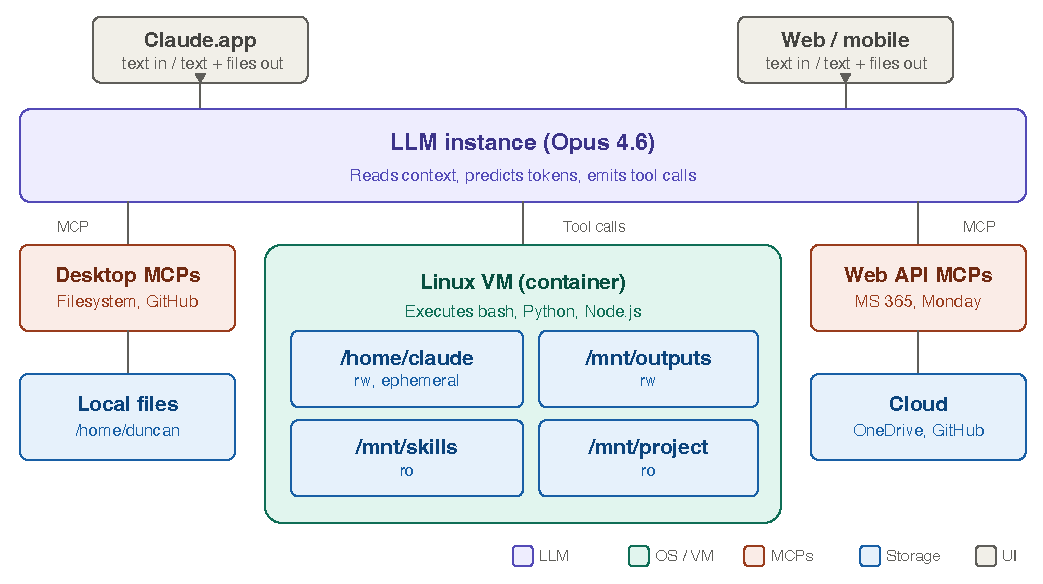
\includegraphics[width=0.95\textwidth]{fig_architecture.pdf}
\caption{Claude runtime architecture. Capabilities only available to the desktop application (Desktop MCPs  such as local file system access) are shown to the left of capabilities that are also available from Web API (the Linux VM and Web API MCPs). The LLM communicates with the Linux VM through tool calls. MCPs (Model Context Protocol connectors) provide authenticated access to external services. Filesystems vary in persistence: \texttt{/home/claude} is ephemeral; \texttt{/mnt/skills} and \texttt{/mnt/project} are read-only and persist across chats.}
\label{fig:architecture}
\end{figure}

The container also contains a compiled binary called \texttt{process\_api} (3.3~MB, statically linked ELF executable), which receives tool calls from the orchestration layer, executes them, and returns results. The LLM inference does \emph{not} happen inside this container. The container is a peripheral device for code execution; the LLM runs on GPU servers elsewhere. The user's text never passes through the container unless the LLM explicitly issues a tool call.

\section{The orchestration harness}
\label{sec:harness}

Between the user interface and the LLM, an orchestration harness manages the conversation lifecycle: context assembly, tokenization (Sec.~\ref{sec:tokenizer}), inference on GPU infrastructure (Sec.~\ref{sec:transformer}), tool routing, and detokenization.

When tool calls are involved, the flow becomes iterative (Fig.~\ref{fig:agent_loop}). Each tool call requires a complete additional pass through the transformer, because the model must process the full context (now including the tool result) to generate its next response. A response involving two tool calls requires at least three transformer passes. The harness has access to information the LLM does not: token counts, proximity to the context limit, rate limits, and user account details. The LLM can only observe what the harness places in the context window. Users can observe compaction through a status bar; the LLM sees only the compacted result.


\begin{figure}
\centering
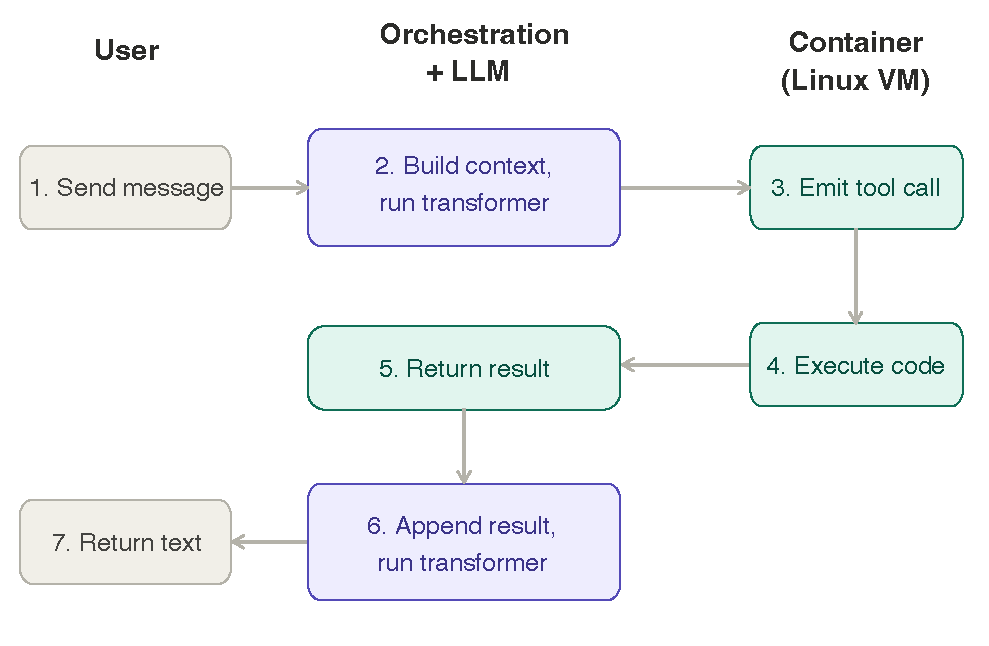
\includegraphics[width=0.95\textwidth]{fig_agent_loop.pdf}
\caption{The agent loop for a tool-using interaction. The user sends a message that the LLM used to write a tool that is called in the Linux container. The code is executed and its result returned to the LLM and appended to the context window. The context window is then run through the transformer and the result returned to the user. Each transformer pass (steps~2, 6) processes the entire context window. Prompt caching~\cite{anthropic_prompt_caching} can reduce the cost of reprocessing unchanged prefixes.}
\label{fig:agent_loop}
\end{figure}


\section{Compaction}
\label{sec:compaction}

When the context window approaches capacity, the harness triggers \emph{compaction}~\cite{anthropic_compaction}: it generates a summary of the conversation, replaces the earlier history with that summary, and drops the originals. The conversation continues from the summary. Compaction is lossy. After compaction, the model may lose access to specific earlier exchanges or exact numerical results from previous tool calls. The system prompt and project instructions are always preserved. 

Importantly, compaction affects the context window, not the stored chat. The full history remains visible to the user in the interface---they can scroll back and read all messages. But the model sees only the compacted summary. The user's view and the model's view diverge after compaction.

\section{The research tool}
\label{sec:research}

One of Claude's most powerful but least-known capabilities is the \textbf{Research} tool~\cite{anthropic_research,anthropic_research_eng}. Unlike a simple web search (where the model makes a single search call and synthesizes results), Research is a multi-agent system that can conduct extended investigations lasting up to 45 minutes, searching across hundreds of sources and producing structured, cited reports.

The architecture, disclosed in Anthropic's June 2025 engineering blog post~\cite{anthropic_research_eng}, uses an orchestrator-worker pattern with two tiers of models (Fig.~\ref{fig:research}). A \emph{LeadResearcher} agent, running on Claude Opus 4, analyzes the user's query, develops a research strategy, and spawns multiple \emph{subagents}, each running on Claude Sonnet 4 with its own independent context window. The subagents execute web searches, evaluate source quality, and compress their findings before returning results to the lead agent. After each batch of subagents completes, the LeadResearcher synthesizes results and decides whether to spawn additional subagents. A \emph{CitationAgent} handles final source attribution.

\begin{figure}
\centering
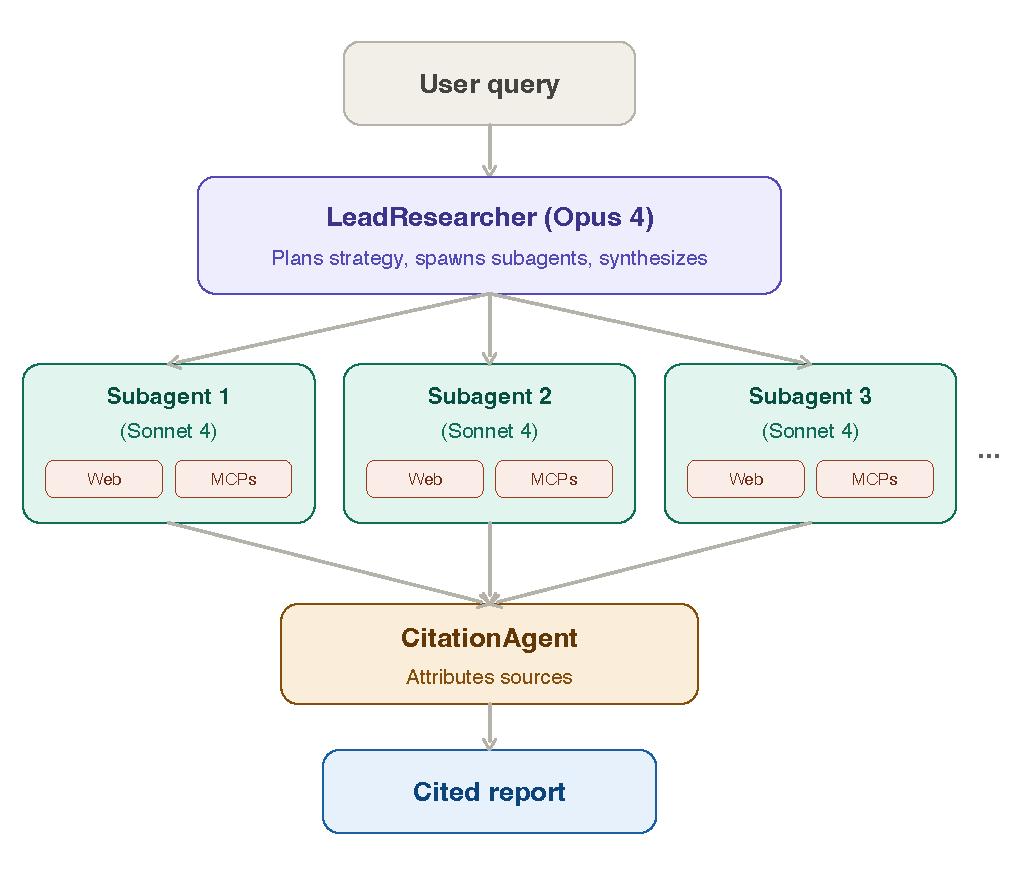
\includegraphics[width=0.95\textwidth]{fig_research.pdf}
\caption{Research tool architecture. The LeadResearcher (Opus 4) orchestrates multiple Sonnet 4 subagents that search in parallel across web and connected MCPs. A CitationAgent attributes sources in the final report. Complex queries may spawn 10+ subagents running for up to 45 minutes.}
\label{fig:research}
\end{figure}

The system scales dynamically: simple fact-finding triggers a single agent with 3--10 tool calls in under two minutes; complex research queries deploy 10+ parallel subagents across hundreds of sources. Importantly, Research can access not only the open web but also any connected MCP integrations (Sec.~\ref{sec:mcp})---including institutional email, shared documents, and enterprise tools---simultaneously. Anthropic reports that the multi-agent system outperforms a single-agent approach by over 90\% on their internal benchmarks~\cite{anthropic_research_eng}. 

Users invoke Research by clicking a toggle in the chat interface. The task runs in the background; the user need not keep the tab open. The output is a structured multi-section report with inline citations linking to original sources. For research administrators, the Research tool is particularly valuable for tasks like policy comparison across peer institutions, literature reviews for strategic planning, regulatory analysis, and any investigation requiring synthesis across many sources. It is qualitatively different from asking Claude a question: it is closer to hiring a research assistant to spend an afternoon in the library.

\section{Tokenization}
\label{sec:tokenizer}

Sections~\ref{sec:analogy}--\ref{sec:research} provide a complete working understanding for most practical purposes. The remaining sections go deeper for readers who wish to understand \emph{how} the LLM generates its responses.

The first step in processing text is \emph{tokenization}: converting characters into integer token IDs. Claude uses a proprietary tokenizer based on Byte-Pair Encoding (BPE)~\cite{sennrich2016bpe}. The vocabulary contains approximately 65,000 tokens for earlier models~\cite{tokenizer_analysis}; the vocabulary for Claude 3+ is undisclosed. Tokens do not correspond to words simply. ``Tokenization'' might become ``token'' + ``ization.'' Numbers and punctuation are tokenized in ways that do not align with human intuition. The tokenizer and model weights are coupled. The embedding layer maps each token ID to a learned vector, and the output layer maps vectors back to probabilities. Changing the tokenizer breaks both layers. This coupling is the deeper reason chats cannot be moved between models (Sec.~\ref{sec:chats}).

\section{The transformer}
\label{sec:transformer}

Claude is built on the \emph{transformer} architecture~\cite{vaswani2017attention}, specifically an autoregressive (decoder-only) variant. The Claude 3 Model Card describes Claude as generating responses ``one set of characters at a time, in order''~\cite{anthropic_model_card}.
The architecture is shown in Fig.~\ref{fig:transformer}. After tokenization, each token is mapped to an \emph{embedding} vector. These pass through a stack of transformer layers, each with two sub-layers:

\begin{figure}
\centering
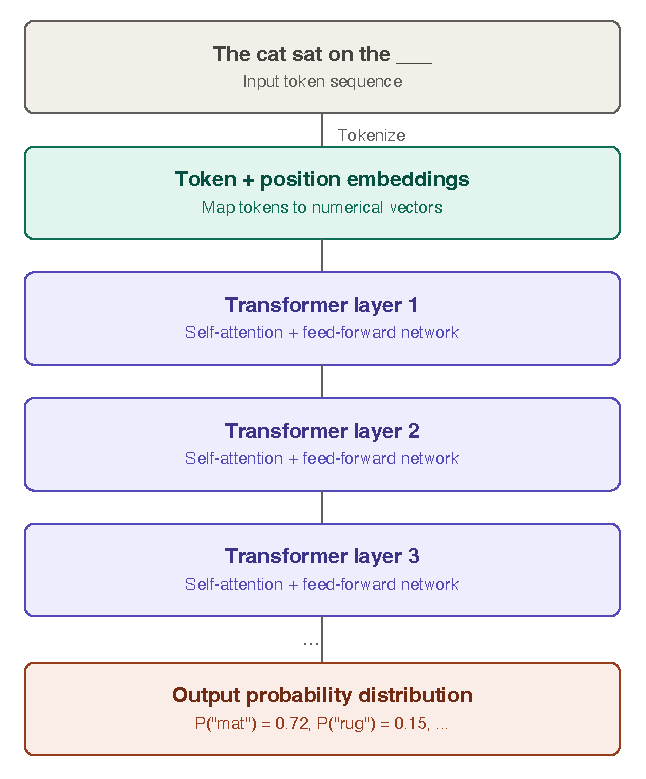
\includegraphics[width=0.48\textwidth]{fig_transformer.pdf}
\caption{Simplified transformer schematic. Input tokens (bottom) are converted to numerical vectors by the embedding layer, which maps discrete token IDs to continuous vectors and is coupled to the tokenizer. These vectors pass through a stack of transformer layers; each layer contains a self-attention mechanism (illustrated by the orange lines between tokens, whose thickness represents attention weight) followed by a feed-forward network that stores factual knowledge and reasoning heuristics in its trained weights. Self-attention allows every token to attend to every other token, with computational cost scaling as $O(n^2)$ with sequence length $n$. The output layer maps the final vectors to a probability distribution over the vocabulary (approximately 65,000 tokens), from which the next token is sampled and appended---a process called autoregressive generation.}
\label{fig:transformer}
\end{figure}

\begin{enumerate}
\item \textbf{Self-attention.} Computes, for each token, a weighted combination of information from all other positions. Attention weights depend on content, allowing the model to capture long-range relationships. Self-attention scales as $O(n^2)$ with sequence length~\cite{vaswani2017attention}; for one million tokens, optimizations such as FlashAttention~\cite{dao2022flashattention} are almost certainly required.

\item \textbf{Feed-forward network.} Each position is processed independently through a multi-layer perceptron, where factual knowledge and reasoning heuristics are stored in trained weights.
\end{enumerate}
After all layers, the final vectors are mapped to probability distributions over the vocabulary. The model samples the next token, appends it, and repeats (\emph{autoregressive} generation). Anthropic trains Claude using JAX, PyTorch, and Triton on Google TPUs, Amazon Trainium chips, and NVIDIA GPUs~\cite{anthropic_model_card}. Parameter counts, layer counts, and architectural details are not publicly disclosed~\cite{scaling_monosemanticity}.

\section{Practical implications}
\label{sec:implications}

\textbf{Never trust a number the LLM produced in prose.} The model predicts plausible-looking tokens, not computed results. All numerical analysis should be performed by Python code on the Linux VM. The skill architecture (Sec.~\ref{sec:skills}) enforces this by routing computation through scripts.

\textbf{Be skeptical of self-knowledge.} Claude cannot reliably report on its own architecture. One model instance fabricated ``54,633 tokens out of 449,000'' with fictional ``token usage warnings.'' Claims about its own architecture derive from training data, not genuine introspection~\cite{anthropic_api_docs}.

\textbf{Understand what costs context.} Every message, tool result, and loaded skill consumes tokens that persist. For extended work, start fresh chats for distinct tasks.

\textbf{Distinguish the model from the harness.} The LLM is one component. The harness manages context, compaction, and tool routing. The container executes code. MCPs access external systems. Failures may occur in any component.

\textbf{Understand model binding.} Conversations cannot transfer between models (Sec.~\ref{sec:chats}). Plan the model choice before beginning complex work.

\textbf{Use projects for serious work.} Project instructions, cross-chat search, scoped memory, and information firewalling (Sec.~\ref{sec:projects}) make projects essential for any multi-session analytical workflow.

\textbf{Use Research for complex investigations.} The Research tool (Sec.~\ref{sec:research}) can search hundreds of sources over tens of minutes, across both the open web and connected enterprise tools. It is qualitatively different from asking a question in chat and is particularly suited to policy comparison, regulatory analysis, and literature reviews.

\section{Conclusion}
\label{sec:conclusion}

We have presented a scaffolded introduction to Claude's architecture. The key insights are: (i) the context window is finite and reconstructed from scratch every turn; (ii) chats persist but are bound to a specific model; (iii) projects provide persistent workspaces with cross-chat search and information separation; (iv) skills route deterministic computation through code; (v) MCP connectors integrate enterprise tools; (vi) the Research tool conducts multi-agent investigations across web and institutional sources; (vii) the LLM generates text statistically; and (viii) the model cannot introspect on its own state.

For further reading: the Anthropic API documentation~\cite{anthropic_api_docs} covers context windows, tool use, and compaction; the Claude 3 Model Card~\cite{anthropic_model_card} describes architecture and training; the ``Scaling Monosemanticity'' paper~\cite{scaling_monosemanticity} explores interpretability; and Vaswani et al.~\cite{vaswani2017attention} and the ``Illustrated Transformer'' (\url{https://jalammar.github.io/illustrated-transformer/}) provide transformer background.

\section*{Acknowledgments}
The author thanks Brett Padgett for the questions that motivated this paper and for the critical observation that prompted examination of which claims about Claude's architecture are verified and which are fabricated.


\subsection*{Disclosure statement}
The author reports there are no competing interests to declare.

\subsection*{Use of generative AI}
This paper was drafted with the assistance of Claude Opus 4.6 (Anthropic, 2026). Claude was used for: (i) drafting and iteratively revising manuscript text based on the author's outlines, corrections, and editorial direction; (ii) writing Python (matplotlib) scripts that produced the schematic figures, which were iteratively refined under the author's direction; (iii) conducting web searches to verify architectural claims against Anthropic's public documentation; and (iv) direct runtime inspection of its own execution environment (filesystem structure, container metadata, process inventory) to obtain architectural details reported in the paper. Claude is both the subject of this paper and a tool used in its preparation. All text was reviewed, edited, and verified by the author against authoritative sources. All figures are deterministic outputs of Python scripts and were reviewed and iteratively revised by the author. Architectural claims were verified against Anthropic's public documentation, API references, and research publications.

\subsection*{Data availability statement}
No datasets were generated or analyzed in this study. Architectural claims are based on publicly available documentation cited in the references and on direct runtime inspection described in the text.

\appendix

\section{Case study: The OSP Budget Template skill}
\label{app:osp}

This appendix describes the Syracuse University OSP Budget Template skill (\texttt{su-osp-budget}), a production skill used by the Office of Research to assist principal investigators with sponsored research budget development. It illustrates how a complex, domain-specific workflow is encoded as a skill, and how the skill architecture separates statistical reasoning from deterministic computation.

When a faculty member prepares a grant proposal for the National Science Foundation, the National Institutes of Health, or another sponsor, they must complete a detailed budget workbook specifying personnel costs (with fringe benefits), equipment, travel, participant support, materials, consultants, subawards, tuition, and indirect costs (facilities and administrative, or F\&A). The budget must comply with federal cost principles (2~CFR~200), sponsor-specific policies (e.g., the NIH salary cap, the NSF two-month rule), and Syracuse University's internal policies (e.g., college-specific tuition remission rates, the current F\&A rate agreement with DHHS).

This is a task where errors are consequential---an incorrect fringe rate or a misapplied F\&A base can result in a budget that is rejected by the sponsor or that commits the university to unrecoverable cost overruns---and where the relevant policies are complex and change frequently.

The \texttt{su-osp-budget} skill (version 2.1, last updated March 2026) occupies 2.6~MB and contains all four skill components:
\begin{enumerate}
\item \texttt{SKILL.md} (29~KB): The entry point. It specifies prerequisites (Claude Opus 4.5 or higher is required), documents the complete budget workbook structure including which cells are writable and which contain protected formulas, encodes all policy rules as natural language instructions, and provides quick-reference rate tables. It also contains version history and explicit instructions for future updates.

\item \texttt{references/} (136~KB, 16 files): Detailed policy documentation organized by topic: personnel guidance, NIH policies, NSF policies, salary policies, tuition policies, subaward rules, participant support rules, consultant/contractor distinctions, human subjects payments, budget justification templates, and a critical file (\texttt{safe\_cells.md}) documenting exactly which cells in the Excel template are safe to write to.

\item \texttt{scripts/} (56~KB, 3 files):
  \begin{itemize}
  \item \texttt{rate\_lookup.py}: Functions for looking up fringe benefit rates by account code, fund type, and fiscal year, and F\&A rates by activity type and location.
  \item \texttt{budget\_calculator.py}: Functions for calculating fully loaded costs, faculty monthly rates, NIH-capped salaries, course buyouts, subaward costs, and multi-year escalation.
  \item \texttt{budget\_population.py} (38~KB): The main script that populates the Excel workbook template, writing values only to safe cells and preserving all formulas.
  \end{itemize}

\item \texttt{assets/} (2.4~MB, 10 files): The OSP Budget Template Excel workbook, fringe rate data files for FY2025 and FY2026, F\&A rate history, GSA per diem rate files, and supporting documentation.
\end{enumerate}

When a PI says ``Create an NSF budget for a 3-year grant with 1 month of summer salary, 2 graduate students, and travel to one conference per year,'' the following sequence occurs:
\begin{enumerate}
\item The LLM reads SKILL.md into its context window. The natural language instructions tell it how to interpret the PI's request, which policy rules apply (NSF two-month rule, federal fringe rates, F\&A at 49.5\%), and which scripts to call.

\item The LLM calls \texttt{rate\_lookup.py} to look up the current fringe rates for faculty summer salary (15.8\%) and graduate assistants on federal grants (10.8\%), and the F\&A rate for on-campus research (49.5\%). These lookups are deterministic---they read from the fringe rate data files in the assets directory.

\item The LLM calls \texttt{budget\_calculator.py} to compute fully loaded costs with escalation across the three-year period.

\item The LLM calls \texttt{budget\_population.py} to populate the Excel workbook template, writing computed values to the safe cells documented in \texttt{safe\_cells.md} while preserving all formula cells.

\item The LLM copies the populated workbook to \texttt{/mnt/user-data/outputs} for the PI to download.
\end{enumerate}
At no point does the LLM ``predict'' a fringe rate or ``guess'' at a salary calculation. Every number in the final budget comes from a deterministic Python computation. The LLM's contribution is understanding the PI's natural language request, mapping it to the correct policy rules, constructing the correct function calls, and producing a clear explanation of the budget for the PI's review.

The skill includes explicit version management. The SKILL.md contains a version history table documenting every change since the initial release in November 2025. It includes auto-increment instructions: when the skill is updated via the skill-creator, the minor version increments automatically (2.1 $\to$ 2.2 $\to$ 2.3), the ``Last Updated'' date is set to the current date, and a new entry is added to the version history. Major version increments (e.g., 2.x $\to$ 3.0) require explicit user instruction.

The skill also includes instructions for maintaining the rate data: when new fiscal year fringe rates are published by the Comptroller, the user adds a new data file (\texttt{fringe\_rates\_by\_account\_fyYYYY.xlsx}) to the assets directory, and the \texttt{rate\_lookup.py} script automatically selects the correct file based on the fiscal year parameter. The skill's documentation includes instructions that tell the skill-creator LLM how to update the source repository in GitHub and rebuild the binary distribution, enabling the skill to be maintained as a versioned software artifact even though its primary ``source code'' is natural language.

The OSP Budget skill illustrates several principles discussed in this paper. The separation between statistical reasoning (interpreting the PI's request, selecting policy rules) and deterministic computation (rate lookups, salary calculations, workbook population) is essential for producing trustworthy output. The skill's self-contained design---all rate data, policy references, and calculation functions are bundled within the skill---means it does not depend on external state that might change between conversations. And the explicit versioning and update instructions mean the skill can be maintained over time as policies change, by a user interacting with an LLM rather than editing code in a traditional development environment.

\bibliographystyle{unsrt}
\bibliography{references}

\end{document}
